\documentclass[12pt,oneside]{book}
\usepackage{geometry}
\geometry{a4paper} 
%\geometry{landscape}
\usepackage[parfill]{parskip}  
\usepackage{graphicx}
\usepackage{subfigure}
%\usepackage[section]{placeins}
\usepackage[below]{placeins}

\usepackage{amssymb}

\usepackage[spanish]{babel}
\usepackage[utf8]{inputenc}
\usepackage[T1]{fontenc}

\usepackage{hyperref}

	\title{\Huge MANUAL DE JUEGO}
	\author {Danny Steven Ponce Marin \and Kevin Ricardo Silva Chavez \and Edwin Hermenejildo Reyes}
	\date{30 de Junio del 2013}

\begin{document}
	
	\maketitle
	\tableofcontents
	
	\chapter{ Introducción.} Sudoku \footnote{\url{http://es.wikipedia.org/wiki/Sudoku}} es un pasatiempo que se publicó por primera vez a finales de la década de 1970 y se popularizó en Japón en 1986, dándose a conocer en el ámbito internacional en 2005 cuando numerosos periódicos empezaron a publicarlo en su sección de pasatiempos. 1 El objetivo del sudoku es rellenar una cuadrícula de 9 *  9 (celdas 81 casillas) dividida en subcuadrículas de 3 x 3 (también llamadas "cajas" o "regiones") con las cifras del 1 al 9 partiendo de algunos números ya dispuestos en algunas de las celdas. Aunque se podrían usar colores, letras, figuras, se conviene en usar números para mayor claridad, lo que importa, es que sean nueve elementos diferenciados, que no se deben repetir en una misma fila, columna o subcuadrícula. Un sudoku está bien planteado si la solución es única. La solución de un sudoku siempre es un cuadrado latino, aunque el recíproco en general no es cierto ya que el sudoku establece la restricción añadida de que no se puede repetir un mismo número en una región.

	\chapter{Instrucciones Para Jugar Sudoku}

	\newpage

		\begin{figure}
			\section{Ventana Principal}
			\begin{center}
				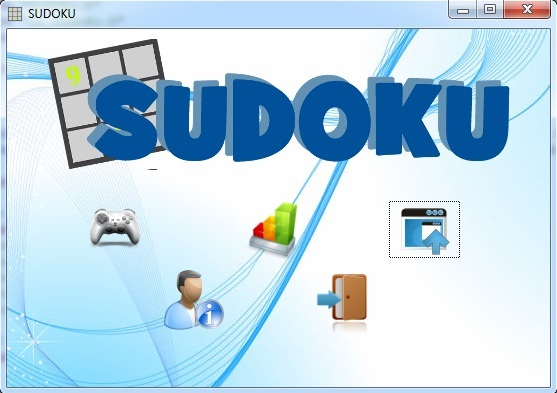
\includegraphics[width=.60\textwidth]{./imagenes/ventanaPrincipal.jpg}
				\caption{Ventana Principal}
				\label{Ventana Principal}
			\end{center}
{\bf Ventana Principal.-} Esta ventana se le presenta al usuario de bienvenida para que pueda a elegir entre: {\bf Nuevo Juego, Estadística, Cargar un juego guardado,  Acerca de y Salir.} \newline El usuario podrá ingresar a cualquiera de las opciones mediante un clic sobre el icono (figura presentada en la ventana).
			\subsection{Nuevo Juego}
Esta ventana se despliega al momento de dar clic en el icono "Nuevo Juego" en la ventana de bienvenida. En esta ventana podemos elegir la dificultad de juego entre : {\bf Fácil, Medio, Difícil y Experto}.
			\begin{center} 
				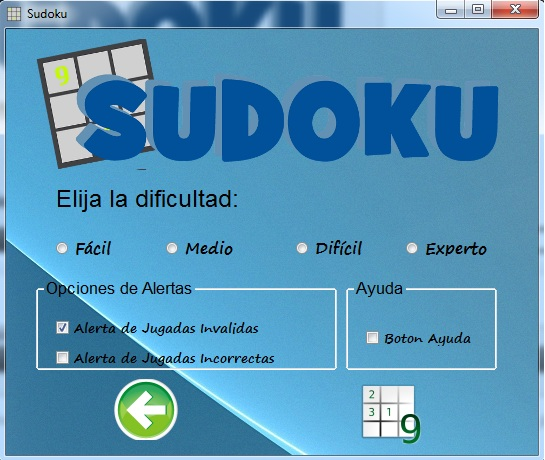
\includegraphics[width=.60\textwidth]{./imagenes/nuevoJuego.jpg}
				\caption{Nuevo Juego}
				\label{Nuevo Juego}
			\end{center}
		\end{figure}
		\begin{figure}
Dependiendo la opción que seleccione el usuario, podra visualizar una ventana de juego similar a las que se muestra a continuación debido a que las casillas se llenan de manera aleatoria en cada nivel de dificultad
		 \ \\ \ \\ \
			\centering
				\subfigure[Fácil]{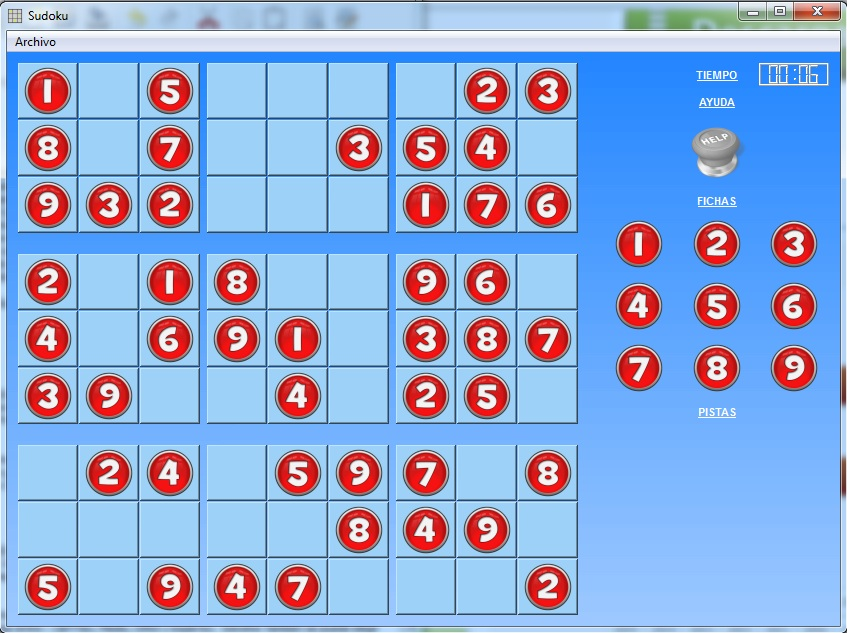
\includegraphics[width=60mm]{./imagenes/facil.jpg}}
				\subfigure[ Medio]{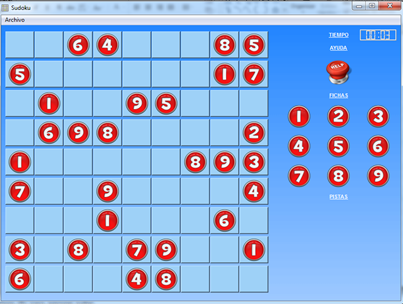
\includegraphics[width=60mm]{./imagenes/medio.jpg}}
				\subfigure[Difícil]{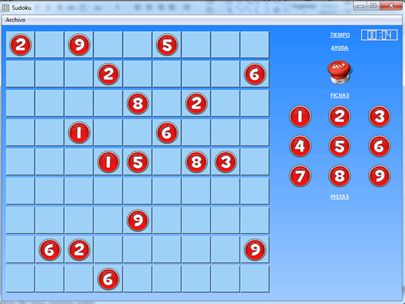
\includegraphics[width=60mm]{./imagenes/dificil.jpg}}
				\subfigure[Experto]{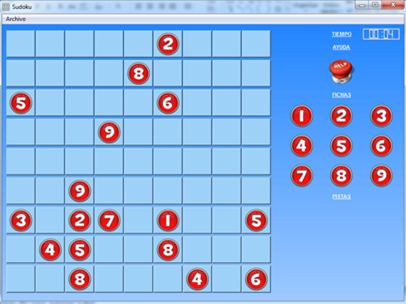
\includegraphics[width=60mm]{./imagenes/experto.jpg}}
				\caption{Niveles de Dificultad.}
		 \ \\ \
		 \begin{flushright} Además el usuario podra activar las {\bf Opciones de Alertas} y {\bf Ayuda} tan solo con dar clic sobre el recuadro(CheckBox) que se encuentra junto al tipo de alerta y ayuda. A continuación se muestra las posibles Alertas que el usuario podra visualizar en caso de realizar movimientos inválidos o movimientos incorrectos.
\end{flushright}
		  \ \\ \ \\ \
			\centering
				\subfigure[Alerta Inválida: Fila]{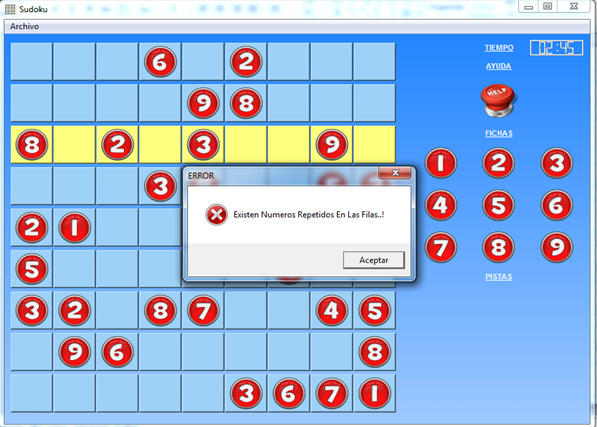
\includegraphics[width=60mm]{./imagenes/alertaFila.jpg}}
				\subfigure[Alerta Inválida: Columna]{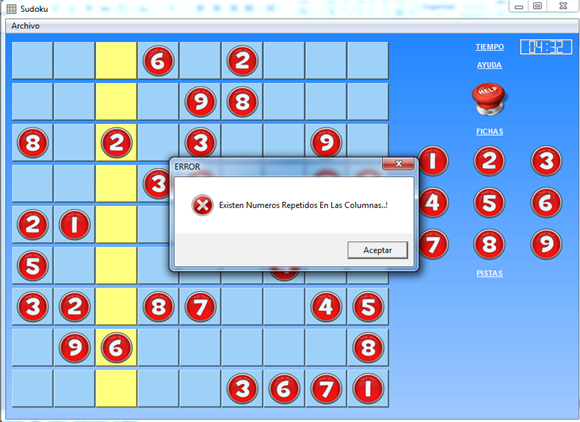
\includegraphics[width=60mm]{./imagenes/alertaColumna.jpg}}
				\subfigure[Alerta Inválida: Sub-Cuadricula]{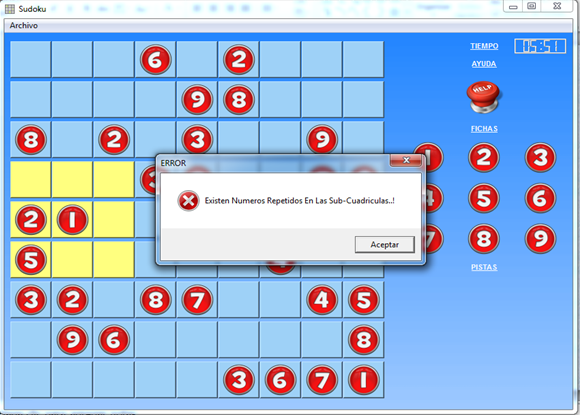
\includegraphics[width=60mm]{./imagenes/alertaSubcuadricula.jpg}}
				\subfigure[Alerta Incorrecta]{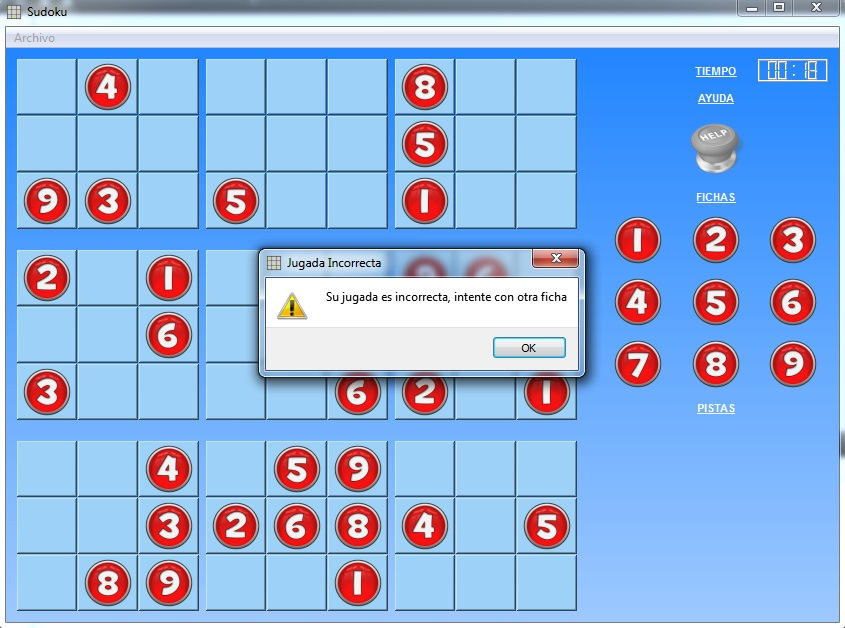
\includegraphics[width=60mm]{./imagenes/alertaIncorrecta.jpg}}
				\caption{Tipos de Alerta.}
		  \ \\ \	
			\subsection{Estadísticas}
			\newpage
Esta ventana se despliega al momento de dar clic en el icono "Estadística" en la ventana de bienvenida. En esta ventana podemos observar el comportamiento general de nuestro juego a lo largo de varias jugadas realizadas y permite identificar la existencia de algún patrón o repetición periódica dentro de nuestro conjunto de resultados.
			
				\begin{center} 
					\includegraphics[width=.60\textwidth]{./imagenes/estadisticas.jpg}
					\caption{Estadistica}
					\label{estadistica}
				\end{center}
			
			\subsection{Cargar Juego}
Nos permite reaundar una partida que a sido guardada previamente por el usuario. Para cargarla damos clic en el icono "Cargar Juego" en la ventana de bienvenida la cual nos despliega una subventana en la cual filtramos(buscamos) con el nombre que se guardo dicha partida. Damos clic en el botón "Aceptar" se despliega la ventana principal de juego y a su ves se reanuda la partida. Como se muestra a continuación.
				\begin{center} 
					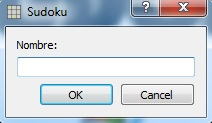
\includegraphics[width=.60\textwidth]{./imagenes/nombre.jpg}
					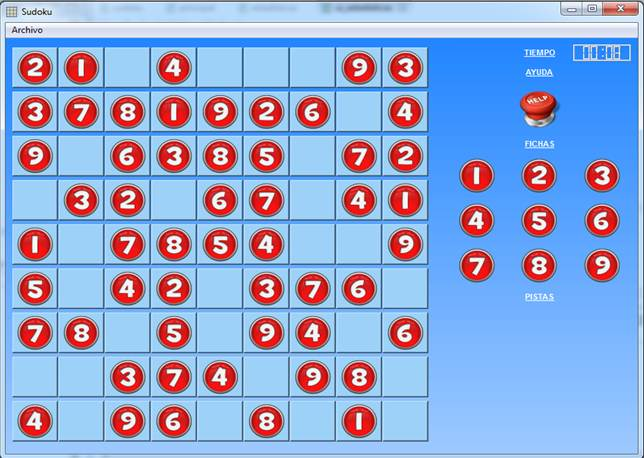
\includegraphics[width=.60\textwidth]{./imagenes/partidaCargada.jpg}
					\caption{Partida Cargada}
					\label{Partida Cargada}
				\end{center}


		\end{figure}
	\chapter{Conclusiones}
		\begin{itemize}
\item Python ofrece buena productividad de programación generalmente un mayor nivel de abstracción.

		\end{itemize}
\end{document}